
\subsection{PB}
\subsubsection{Primo Incremento}

\paragraph{Consuntivo Orario}
\begin{center}
	\renewcommand{\arraystretch}{1.8} %aumento ampiezza righe
	\begin{tabular}{ |m{8em}|c|c|c|c|c|c|c| }
	\hline
	\textbf{Membro} & \textbf{Re} & \textbf{Am} &  \textbf{An} &  \textbf{Pt} &  \textbf{Pg} &  \textbf{Ve} &  \textbf{Totale}\\
    \hline
    Irene Benetazzo   & - & 1 (+1)  & 3 (+3)  & 5 (-3)  & 5       & 4 (+1)  & \textbf{18} (+2) \\
    \hline
    Tommaso Berlaffa  & 3 & -       & 1 (+1)  & -       & 8 (-2)  & 1 (+1)  & \textbf{13} \\
    \hline
    Mattia Episcopo   & - & 3 (-1)  & 2 (+2)  & 7       & 4       & 2       & \textbf{18} (+1) \\
    \hline
    Pietro Macrì      & - & - (-4)  & -       & 6 (+1)  & 6 (-1)  & 2       & \textbf{14} (-4)\\
    \hline
    Qi Fan Andrea Pan & - & -       & -       & 8 (+1)  & 6 (-1)  & 2  (-1) & \textbf{16} (-1) \\
    \hline
    Matteo Pillon     & - & -       & -       & 6 (+1)  & 6 (-2)  & 2  (-1) & \textbf{14} (-2) \\
    \hline
    Samuele Rizzato   & - & 2 (+2)  & 2 (+2)  & 6 (-2)  & 5       & 2  (-1) & \textbf{17} (+1) \\
    \hline
    \textbf{Totale ore} & \textbf{3} & \textbf{8} & \textbf{8} (+8) &  \textbf{38} (-2) &  \textbf{40} (-6) &  \textbf{15} (-1) &  \textbf{110} (-3)\\
    \hline
	\end{tabular}
\end{center}
\begin{figure}[H]
    \centering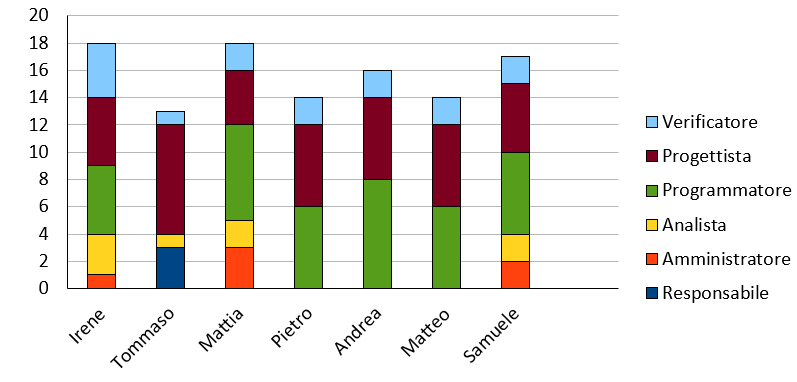
\includegraphics[width=\textwidth, height=\textheight,keepaspectratio]{images/consuntivo/PB-ore.png}
    \caption{PB - Product Baseline - Primo Incremento - consuntivo ripartizione oraria}
\end{figure}

\paragraph{Consuntivo Economico}
\begin{center}
	\renewcommand{\arraystretch}{1.8}
	\begin{tabular}{ |m{6em}|c|c|c|c|c|c|c| }
	\hline
	\textbf{Ruolo} & \textbf{Re} & \textbf{Am} &  \textbf{An} &  \textbf{Pt} &  \textbf{Pg} &  \textbf{Ve} &  \textbf{Totale}\\
    \hline
    Totale ore & 3 & 8 & 8 & 38 & 40 & 14 & \textbf{110}\\
    \hline
    Costo \euro/h & 30\euro/h & 20\euro/h & 25\euro/h & 25\euro/h & 15\euro/h & 15\euro/h & \\
    \hline
    \textbf{Totale costo} & \textbf{90\euro} & \textbf{120\euro} &  \textbf{200\euro} & \textbf{950\euro} &  \textbf{600\euro} &  \textbf{225\euro} &  \textbf{2185\euro} \\
    &  & (-40\euro) & (+200\euro) & (-50\euro) & (-90\euro) & (-25\euro) & (+5\euro) \\
    \hline
	\end{tabular}

    \begin{figure}[H]
        \centering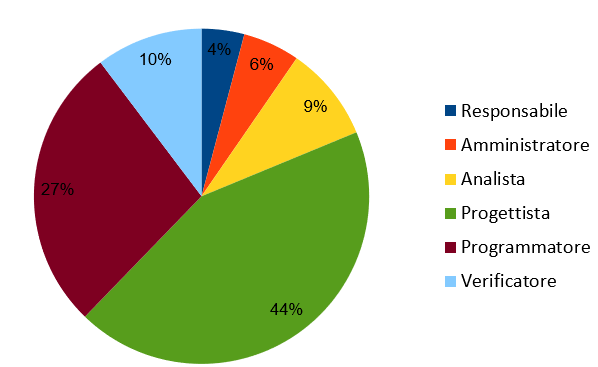
\includegraphics[width=0.7\textwidth, height=0.7\textheight, keepaspectratio]{images/consuntivo/PB-costo.png}
        \caption{PB - Product Baseline - Primo Incremento - consuntivo ripartizione economica}
    \end{figure}
\end{center}

\paragraph{Considerazioni} \hfill \break
L'inizio della fase è stato posticipato, causa revisione con i docenti. A seguito di quest'ultima, 
sono state necessarie ulteriori ore di analista per gestire la correzione e l'analisi di possibili soluzioni della documentazione presentata durante colloquio.\\
L'intera fase di Product Baseline viene quindi temporalmente traslata di conseguenza.

\begin{center}
	\renewcommand{\arraystretch}{1.8}
	\begin{tabular}{ | l |c|c| }
    \hline
    & \textbf{Ore} & \textbf{Costo} \\
	\hline
    \textbf{Consuntivo} & 110 & 2185\euro \\
    \hline
    \textbf{Preventivo} & 113 & 2180\euro \\
    \hline
    \textbf{Bilancio fase} & -3 & +5\euro \\
    \hline
    \textbf{Bilancio complessivo*} & \textbf{8} & \textbf{+15\euro} \\
    \hline
    \end{tabular}
\end{center}
*N.B. Per il bilancio complessivo si considera a partire dal nuovo preventivo a finire in cui le ore sono state azzerate mentre economicamente c'è stato il risparmio di 250\euro.
E' stata necessaria una fase aggiuntiva durante la revisione RTB e quelle variazioni +11ore e +10\euro fanno parte di questo bilancio complessivo. \newline
Rispetto a quanto pianificato il primo incremento ha riguardato più una fase di progettazione e implementazione generale rispetto alle specifiche funzionalità (Requisiti obbligatori). Questo non ha portato a grandi variazioni in termini di ore e costi, ma ha prolungato la fase in durata complessiva e ha cambiato gli obiettivi dell'incremento.
In conclusione il primo incremento della fase Product Baseline termina il 2022-07-20 con un esborso, relativo
alla fase, di 5€.

\newpage

\subsubsection{Secondo Incremento}

\paragraph{Consuntivo Orario}
\begin{center}
	\renewcommand{\arraystretch}{1.8} %aumento ampiezza righe
	\begin{tabular}{ |m{8em}|c|c|c|c|c|c|c| }
	\hline
	\textbf{Membro} & \textbf{Re} & \textbf{Am} &  \textbf{An} &  \textbf{Pt} &  \textbf{Pg} &  \textbf{Ve} &  \textbf{Totale}\\
    \hline
    Irene Benetazzo   & - & -  & -  & 7  & 5 & 2 (-1) & \textbf{14} \\
    \hline
    Tommaso Berlaffa  & - & - & -  & 6 & 6  & 2 (-1) & \textbf{14} \\
    \hline
    Mattia Episcopo   & 3 & -  & -  & - & 10 & 0 & \textbf{13} \\
    \hline
    Pietro Macrì      & - & -  & - & 5 & 6 & 2 (-1) & \textbf{13} \\
    \hline
    Qi Fan Andrea Pan & - & 2 (-2) & - & 4 & 8 & 2 (-1) & \textbf{16} \\
    \hline
    Matteo Pillon     & - & - & - & 6 & 7 & 2 (-1) & \textbf{15} \\
    \hline
    Samuele Rizzato   & - & 3 (-2) & - & 6 & 5 & 2 (-1) & \textbf{16} \\
    \hline
    \textbf{Totale ore} & \textbf{3} & \textbf{5} (-4) & \textbf{0} &  \textbf{34} &  \textbf{47} &  \textbf{12} (-5) &  \textbf{101} (-9)\\
    \hline
	\end{tabular}
\end{center}
\begin{figure}[H]
    \centering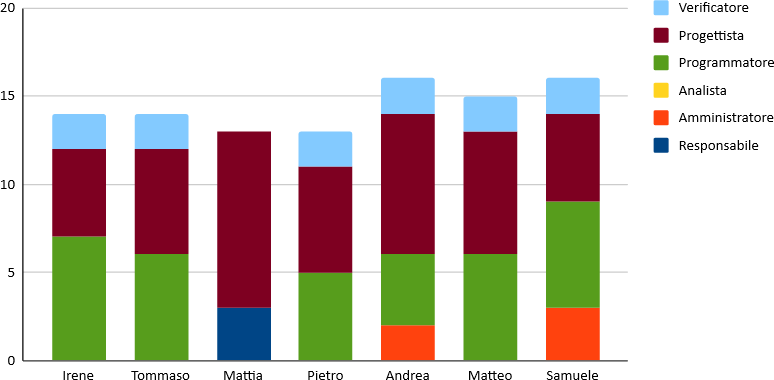
\includegraphics[width=\textwidth, height=\textheight,keepaspectratio]{images/consuntivo/consuntivo-PB-ore-secondo-incremento.png}
    \caption{PB - Product Baseline - Secondo Incremento - consuntivo ripartizione oraria}
\end{figure}

\paragraph{Consuntivo Economico}
\begin{center}
	\renewcommand{\arraystretch}{1.8}
	\begin{tabular}{ |m{6em}|c|c|c|c|c|c|c| }
	\hline
	\textbf{Ruolo} & \textbf{Re} & \textbf{Am} &  \textbf{An} &  \textbf{Pt} &  \textbf{Pg} &  \textbf{Ve} &  \textbf{Totale}\\
    \hline
    Totale ore & 3 & 5 & 0 & 34 & 47 & 12 & \textbf{101}\\
    \hline
    Costo \euro/h & 30\euro/h & 20\euro/h & 25\euro/h & 25\euro/h & 15\euro/h & 15\euro/h & \\
    \hline
    \textbf{Totale costo} & \textbf{90\euro} & \textbf{100\euro} &  \textbf{0\euro} & \textbf{850\euro} &  \textbf{705\euro} &  \textbf{180\euro} &  \textbf{1925\euro} \\
    &  & (-80\euro) & & & & (-75\euro) & (-155\euro) \\
    \hline
	\end{tabular}

    \begin{figure}[H]
        \centering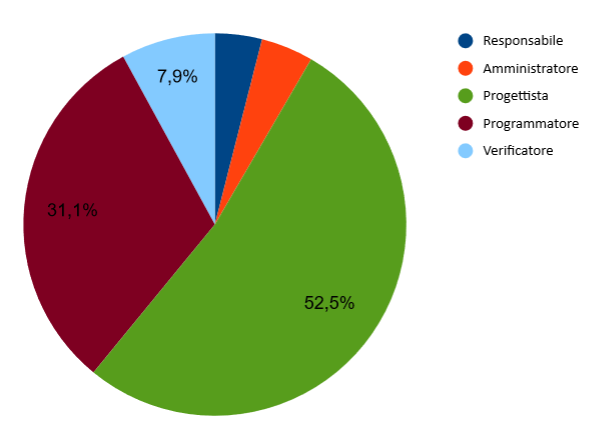
\includegraphics[width=0.7\textwidth, height=0.7\textheight, keepaspectratio]{images/consuntivo/consuntivo-PB-costo-secondo-incremento.png}
        \caption{PB - Product Baseline - Secondo Incremento - consuntivo ripartizione economica}
    \end{figure}
\end{center}

\paragraph{Considerazioni} \hfill \break
Il secondo incremento era stato sovrastimato in sede di preventivo, sia come ore che come costi. In termini di ore c'è stato un discreto risparmio di tempo per i ruoli di verificatore (4) e amministratore (5) che hanno portato ad un risparmio complessivo di 9 ore.
\begin{center}
	\renewcommand{\arraystretch}{1.8}
	\begin{tabular}{ | l |c|c| }
    \hline
    & \textbf{Ore} & \textbf{Costo} \\
	\hline
    \textbf{Consuntivo} & 101 & 1925\euro \\
    \hline
    \textbf{Preventivo} & 110 & 2080\euro \\
    \hline
    \textbf{Bilancio fase} & -9 & -155\euro \\
    \hline
    \textbf{Bilancio complessivo} & \textbf{-1} & \textbf{-140\euro} \\
    \hline
    \end{tabular}
\end{center}
Questo incremento è stato in linea con la pianificazione, in quanto si è entrati nell'implementazione delle specifiche funzionalità. Infatti le ore di progettazione e programmazione sono state correttamente stimate. 
In conclusione il secondo incremento della fase Product Baseline termina il 2022-08-03 con un risparmio economico, relativo alla fase, di 155€.

\subsubsection{Terzo Incremento}

\paragraph{Consuntivo Orario}
\begin{center}
	\renewcommand{\arraystretch}{1.8} %aumento ampiezza righe
	\begin{tabular}{ |m{8em}|c|c|c|c|c|c|c| }
	\hline
	\textbf{Membro} & \textbf{Re} & \textbf{Am} &  \textbf{An} &  \textbf{Pt} &  \textbf{Pg} &  \textbf{Ve} &  \textbf{Totale}\\
    \hline
    Irene Benetazzo   & - & - & - & 4 & 5 & 3 & \textbf{12} \\
    \hline
    Tommaso Berlaffa  & - & - & - & 5 & 4 & 3 & \textbf{12} \\
    \hline
    Mattia Episcopo   & - & 5 & - & 3 & 5 & 2 & \textbf{15} \\
    \hline
    Pietro Macrì      & 3 & - & - & - & 7 & - & \textbf{10} \\
    \hline
    Qi Fan Andrea Pan & - & - & - & 4 & 5 & 3 & \textbf{12} \\
    \hline
    Matteo Pillon     & - & 4 & - & 5 & 3 & 2 & \textbf{14} \\
    \hline
    Samuele Rizzato   & - & - & - & 5 & 5 & 3 & \textbf{13} \\
    \hline
    \textbf{Totale ore} & \textbf{3} & \textbf{9} & \textbf{0} & \textbf{26} & \textbf{34} & \textbf{16} & \textbf{88} \\
    \hline
	\end{tabular}
\end{center}
\begin{figure}[H]
    \centering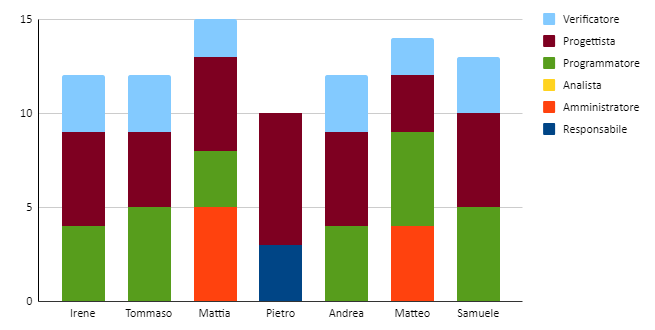
\includegraphics[width=\textwidth, height=\textheight,keepaspectratio]{images/consuntivo/consuntivo-PB-ore-terzo-incremento.png}
    \caption{PB - Product Baseline - Terzo Incremento - consuntivo ripartizione oraria}
\end{figure}

\paragraph{Consuntivo Economico}
\begin{center}
	\renewcommand{\arraystretch}{1.8}
	\begin{tabular}{ |m{6em}|c|c|c|c|c|c|c| }
	\hline
	\textbf{Ruolo} & \textbf{Re} & \textbf{Am} &  \textbf{An} &  \textbf{Pt} &  \textbf{Pg} &  \textbf{Ve} &  \textbf{Totale}\\
    \hline
    Totale ore & 3 & 9 & 0 & 26 & 34 & 16 & \textbf{88}\\
    \hline
    Costo \euro/h & 30\euro/h & 20\euro/h & 25\euro/h & 25\euro/h & 15\euro/h & 15\euro/h & \\
    \hline
    \textbf{Totale costo} & \textbf{90\euro} & \textbf{180\euro} &  \textbf{0\euro} & \textbf{650\euro} &  \textbf{510\euro} &  \textbf{240\euro} &  \textbf{1670\euro} \\
    \hline
	\end{tabular}

    \begin{figure}[H]
        \centering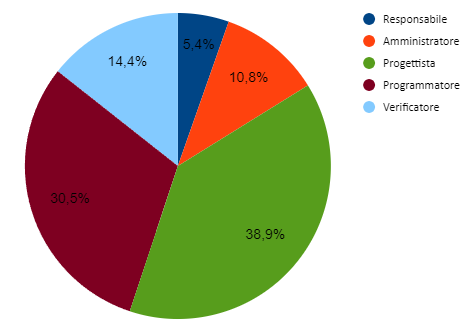
\includegraphics[width=0.7\textwidth, height=0.7\textheight, keepaspectratio]{images/consuntivo/consuntivo-PB-costo-terzo-incremento.png}
        \caption{PB - Product Baseline - Terzo Incremento - consuntivo ripartizione economica}
    \end{figure}
\end{center}

\paragraph{Considerazioni} \hfill \break
Il terzo incremento era stato correttamente stimato in sede di preventivo, sia in termini di numero di ore sia 
in termini di distribuzione delle ore. Il consuntivo di questo incremento si conclude dunque in pari.
\begin{center}
	\renewcommand{\arraystretch}{1.8}
	\begin{tabular}{ | l |c|c| }
    \hline
    & \textbf{Ore} & \textbf{Costo} \\
	\hline
    \textbf{Consuntivo} & 88 & 1670\euro \\
    \hline
    \textbf{Preventivo} & 88 & 1670\euro \\
    \hline
    \textbf{Bilancio fase} & 0 & 0\euro \\
    \hline
    \textbf{Bilancio complessivo} & \textbf{-1} & \textbf{-140\euro} \\
    \hline
    \end{tabular}
\end{center}
Per questo incremento era stata pianificata l'implementazione dei requisiti desiderabili, ma visti i ritardi che si sono accumulati, soprattutto dal punto di vista progettuale, si è optato per svolgerli solo in parte e dare la precedenza a concludere invece i requisiti obbligatori. Questo però non ha comportato gandi differenze in termini di ore e costi e non ha nemmeno avuto impatto sulla durata totale dell'incremento.
In conclusione il terzo incremento della fase Product Baseline termina il 2022-08-17 in pari.
\newpage

\subsubsection{Quarto Incremento}

\paragraph{Consuntivo Orario}
\begin{center}
	\renewcommand{\arraystretch}{1.8} %aumento ampiezza righe
	\begin{tabular}{ |m{8em}|c|c|c|c|c|c|c| }
	\hline
	\textbf{Membro} & \textbf{Re} & \textbf{Am} &  \textbf{An} &  \textbf{Pt} &  \textbf{Pg} &  \textbf{Ve} &  \textbf{Totale}\\
    \hline
    Irene Benetazzo   & 1 (+1) & 2 (-3)  & - & 4 & 4 & 2 & \textbf{13} (-2) \\
    \hline
    Tommaso Berlaffa  & 1 & 3 (-1)  & - & 6 (+2) & 4 & 3 & \textbf{17} (+1) \\
    \hline
    Mattia Episcopo   & 1 & - & - & 4 (-1) & 3 (-1) & 3 & \textbf{11} (-2) \\
    \hline
    Pietro Macrì      & 1 & - & - & 7 (+1) & 7 (+2) & 3 & \textbf{18} (+3) \\
    \hline
    Qi Fan Andrea Pan & 1 & - & - & 5 (+1) & 5 & 3 & \textbf{14} (+1)\\
    \hline
    Matteo Pillon     & 4 (+1) & 0 (-2)  & - & - & 7 & - & \textbf{11} (-1) \\
    \hline
    Samuele Rizzato   & 1 & - & 3 (+3) & 3 (-1) & 5 & 2 (-1) & \textbf{14} (+1) \\
    \hline
    \textbf{Totale ore} & \textbf{10} (+2) & \textbf{5} (-6) & \textbf{3} (+3) & \textbf{29} (+2) & \textbf{35} (+1) & \textbf{16} (-1) & \textbf{98} (+1)\\
    \hline
	\end{tabular}
\end{center}
\begin{figure}[H]
    \centering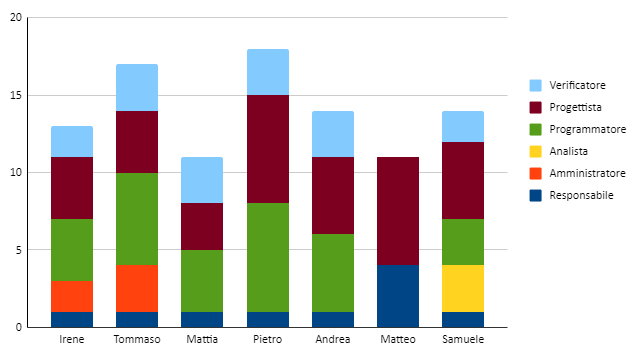
\includegraphics[width=\textwidth, height=\textheight,keepaspectratio]{images/consuntivo/PB-incremento4-orario.png}
    \caption{PB - Product Baseline - Quarto Incremento - consuntivo ripartizione oraria}
\end{figure}
\newpage

\paragraph{Consuntivo Economico}
\begin{center}
	\renewcommand{\arraystretch}{1.8}
	\begin{tabular}{ |m{6em}|c|c|c|c|c|c|c| }
	\hline
	\textbf{Ruolo} & \textbf{Re} & \textbf{Am} &  \textbf{An} &  \textbf{Pt} &  \textbf{Pg} &  \textbf{Ve} &  \textbf{Totale}\\
    \hline
    Totale ore & 10 & 5 & 3 & 29 & 35 & 16 & \textbf{98}\\
    \hline
    Costo \euro/h & 30\euro/h & 20\euro/h & 25\euro/h & 25\euro/h & 15\euro/h & 15\euro/h & \\
    \hline
    \textbf{Totale costo} & \textbf{300\euro} & \textbf{100\euro} &  \textbf{75\euro} & \textbf{725\euro} &  \textbf{525\euro} &  \textbf{240\euro} &  \textbf{1965\euro} \\
    & (+60\euro) & (-120\euro) & (+75\euro) & (+50\euro) & (+15\euro) & (-15\euro) & (+65\euro) \\
    \hline
	\end{tabular}

    \begin{figure}[H]
        \centering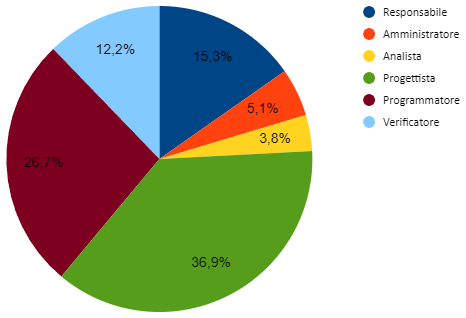
\includegraphics[width=0.7\textwidth, height=0.7\textheight, keepaspectratio]{images/consuntivo/PB-incremento4-costo.png}
        \caption{PB - Product Baseline - Quarto Incremento - consuntivo ripartizione economica}
    \end{figure}
\end{center}

\paragraph{Considerazioni} \hfill \break
Il quarto incremento non è stato correttamente stimato in sede di preventivo, sia in termini di numero di ore sia 
in termini di distribuzione delle ore. Il consuntivo di questo incremento si conclude dunque con l'utilizzo di 12 ore in più rispetto al preventivo, aventi un costo totale per questa fase di 270\euro.
\begin{center}
	\renewcommand{\arraystretch}{1.8}
	\begin{tabular}{ | l |c|c| }
    \hline
    & \textbf{Ore} & \textbf{Costo} \\
	\hline
    \textbf{Consuntivo} & 109 & 2170\euro \\
    \hline
    \textbf{Preventivo} & 97 & 1900\euro \\
    \hline
    \textbf{Bilancio fase} & +12 & +270\euro \\
    \hline
    \textbf{Bilancio complessivo} & \textbf{+11} & \textbf{+130\euro} \\
    \hline
    \end{tabular}
\end{center}
Nel corso di questo incremento si sono svolte attività per lo più di implementazione e testing, per concludere il prodotto in tutte le sue funzionalità e prepararlo per l'ultima fase. Questo in termini di ore ha inciso poco però ha cambiato la struttura dell'incremento rispetto a come era stato pianificato.
In conclusione il quarto incremento della fase Product Baseline termina il 2022-08-30 con un costo economico, relativo alla fase, di 270\euro.

\subsubsection{Complessivo PB}

\paragraph{Consuntivo Orario}
\begin{center}
	\renewcommand{\arraystretch}{1.8} %aumento ampiezza righe
	\begin{tabular}{ |m{8em}|c|c|c|c|c|c|c| }
	\hline
	\textbf{Membro} & \textbf{Re} & \textbf{Am} &  \textbf{An} &  \textbf{Pt} &  \textbf{Pg} &  \textbf{Ve} &  \textbf{Totale}\\
    \hline
    Irene Benetazzo   & 1 & 3 & 3 & 20 & 19 & 11 & \textbf{57} \\
    \hline
    Tommaso Berlaffa  & 4 & 3 & 1 & 17 & 22 & 9 & \textbf{56} \\
    \hline
    Mattia Episcopo   & 4 & 8 & 2 & 14 & 22 & 7 & \textbf{57} \\
    \hline
    Pietro Macrì      & 4 & 0 & 0 & 18 & 26 & 7 & \textbf{55} \\
    \hline
    Qi Fan Andrea Pan & 1 & 2 & 0 & 21 & 24 & 10 & \textbf{58} \\
    \hline
    Matteo Pillon     & 4 & 4 & 0 & 17 & 23 & 6 & \textbf{54} \\
    \hline
    Samuele Rizzato   & 1 & 5 & 5 & 20 & 20 & 9 & \textbf{60} \\
    \hline
    \textbf{Totale ore} & \textbf{19} & \textbf{25} & \textbf{11} & \textbf{127} & \textbf{156} & \textbf{59} & \textbf{397} \\
    \hline
	\end{tabular}
\end{center}
\begin{figure}[H]
    \centering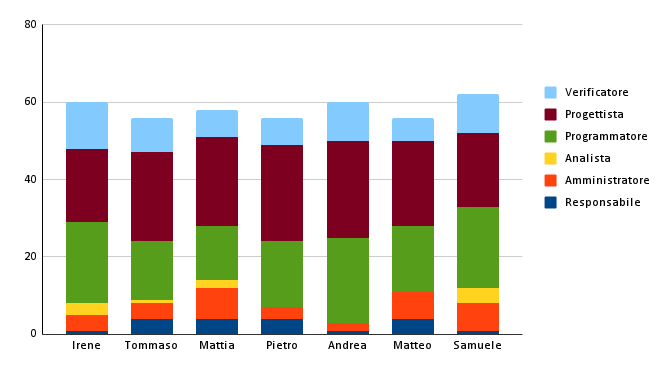
\includegraphics[width=\textwidth, height=\textheight,keepaspectratio]{images/consuntivo/consuntivo-PB-ore-totale.png}
    \caption{PB - Product Baseline - Complessivo PB - consuntivo ripartizione oraria}
\end{figure}
\newpage

\paragraph{Consuntivo Economico}
\begin{center}
	\renewcommand{\arraystretch}{1.8}
	\begin{tabular}{ |m{6em}|c|c|c|c|c|c|c| }
	\hline
	\textbf{Ruolo} & \textbf{Re} & \textbf{Am} &  \textbf{An} &  \textbf{Pt} &  \textbf{Pg} &  \textbf{Ve} &  \textbf{Totale}\\
    \hline
    Totale ore & 19 & 25 & 11 & 127 & 156 & 59 & \textbf{397}\\
    \hline
    Costo \euro/h & 30\euro/h & 20\euro/h & 25\euro/h & 25\euro/h & 15\euro/h & 15\euro/h & \\
    \hline
    \textbf{Totale costo} & \textbf{570\euro} & \textbf{500\euro} &  \textbf{275\euro} & \textbf{3175\euro} &  \textbf{2340\euro} &  \textbf{885\euro} &  \textbf{7745\euro} \\
    \hline
	\end{tabular}

    \begin{figure}[H]
        \centering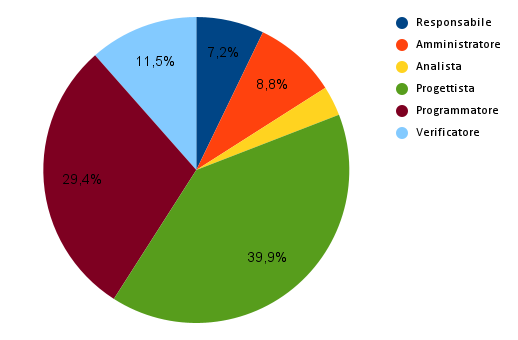
\includegraphics[width=0.7\textwidth, height=0.7\textheight, keepaspectratio]{images/consuntivo/consuntivo-PB-costo-totale.png}
        \caption{PB - Product Baseline - Complessivo PB - consuntivo ripartizione economica}
    \end{figure}
\end{center}

\paragraph{Considerazioni} \hfill \break
\begin{center}
	\renewcommand{\arraystretch}{1.8}
	\begin{tabular}{ | l |c|c| }
    \hline
    & \textbf{Ore} & \textbf{Costo} \\
	\hline
    \textbf{Consuntivo} & 397 & 7745\euro \\
    \hline
    \textbf{Preventivo} & 408 & 7830\euro \\
    \hline
    \textbf{Bilancio macrofase} & -11 & -85\euro \\
    \hline
    \end{tabular}
\end{center}
La Product Baseline termina il 2022-08-30 con un ritardo di 35 giorni rispetto alla pianificazione, 15 dei quali dovuti alla precedente revisione RTB che ha richiesto una fase aggiuntiva non prevista e 20 dovuti a ritardi nell'avanzamento del lavoro. Rispetto alla pianificazione del lavoro di questa macrofase, si sono conclusi tutti i requisiti obbligatori mentre i requisiti desiderabili sono stati portati a termine solo in parte. In questa macrofase nonostante i giorni in più c'è stato un lieve risparmio sia numerico che economico ma considerando la fase aggiuntiva della precedente macrofase si è in pari con le ore e c'è un esborso economico di 180\euro.

\newpage
\paragraph{Preventivo a Finire} \hfill \break

\begin{center}
	\renewcommand{\arraystretch}{1.8}
	\begin{tabular}{ | l |c|c|c| }
    \hline
    \textbf{Ruolo} & \textbf{Nuovo per CA} & \textbf{Precedente per CA}  & \textbf{Differenza economica}\\
	\hline
    \textbf{Responsabile} & 5 & 10 & -150\euro \\
    \hline
    \textbf{Amministratore} & 10 & 10 & 0\euro \\
    \hline
    \textbf{Analista} & 0 & 0 & 0\euro \\
    \hline
    \textbf{Progettista} & 10 & 10 & 0\euro \\
    \hline
    \textbf{Programmatore} & 10 & 10 & 0\euro \\
    \hline
    \textbf{Verificatore} & 65 & 60 & +75\euro \\
    \hline
    \textbf{Totale} & \textbf{100} & \textbf{100} & \textbf{-75\euro} \\
    \hline
    \end{tabular}
\end{center}
Il preventivo a finire ha subito un solo spostamento di 5 ore dal ruolo responsabile a verificatore perchè si prevede maggiore necessità di testare il prodotto; ciò comporterebbe un ipotetico risparmio di 75\euro.